\section{Esercizio 2}
Lo scopo del secondo esercizio serve a gestire:
\begin{enumerate}
\item  identificatori/funzioni non dichiarati
\item  identificatori/funzioni dichiarate più volte nello stesso ambiente
\end{enumerate}

\subsection{Symbol Table}
\label{sec:symboltable}
Per soddisfare i punti elencati precedentemente viene utilizzata una symbol table (ST) con struttura invariata rispetto a quella di SimpLanPlus fornito come modello. Gli attributi e i metodi della classe \textit{SymbolTable} sono mostrati in Figura \ref{fig:STstructure}. Tale struttura implementa una lista di HashMap per la gestione degli ambienti della symbol table. Ogni HashMap è costruita fornendo come chiave una stringa contenente l'identificativo \textit{id} della variabile o della funzione e da un oggetto STentry che contiene le informazioni dell'elemento con identificativo \textit{id}. 

\begin{figure}[h]
\centering
\begin{subfigure}{.45\textwidth}
  \centering
  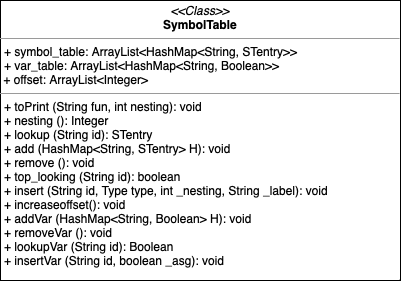
\includegraphics[width=1\linewidth]{Images/ST_structure.png}
  \caption{Struttura della classe SymbolTable}
  \label{fig:STstructure}
\end{subfigure}
\begin{subfigure}{.45\textwidth}
  \centering
  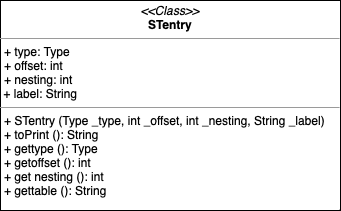
\includegraphics[width=1\linewidth]{Images/STentry _structure.png}
  \caption{Struttura della classe STentry}
  \label{fig:STentrystructure}
\end{subfigure}
\end{figure}

La struttura di STentry contiene i metodi e i campi mostrati in Figura \ref{fig:STentrystructure}, dove:
\begin{itemize}
    \item \textbf{type} è il tipo della varibile o della funzione, dove nel primo caso i tipi ammessi sono int, bool e void, mentre nel secondo caso ho un un tipo \textit{ArrowType} costruito nel modo seguente. Dove \textit{inputtype} è la lista che contiene i tipi dei parametri in input e \textit{outputtype} è il tipo dell'output della funzione, che può essere anch'esso int, bool e void.
    \begin{minted}[xleftmargin=20pt,linenos]{java}
    public class ArrowType extends Type {
	   private ArrayList<Type> inputtype; 
	   private Type outputtype;
    ...
    }
    \end{minted}
    \item \textbf{offset} è un numero intero che indica l'offset di quella variabile o funzione in quell'ambiente.
    \item \textbf{nesting} è un numero intero che indica il livello di nesting nella quale la variabile o funzione è stata dichiarata.
    \item \textbf{label} è una stringa che, nel caso delle variabili è vuota (""), nel caso delle funzioni contiene l'etichetta assegnata a quella funzione da utilizzare in fase di code generation.
\end{itemize}

Per quanto riguarda gli oggetti \textit{$var_table$} e \textit{offset} servono a gestire rispettivamente le variabili dichiarate ma non assegnate e l'assegnamento degli offset. Più informazioni riguardanti la Var Table (VT) sono presenti nella Sezione \ref{sec:vartable}.

Di seguito viene mostrato un esempio del funzionamento della ST.

\begin{minted}[xleftmargin=20pt,linenos]{java}
int a ;
int b ;
int g(int p){
    int y ;
    y = 2;
    p+y
}
int f(int n){
    int b ;
    b = 3;
    g(b+n)
}
a = 1;
b = 2 ;
f(a) ;
\end{minted}

\begin{figure}[h]
\centering
\begin{subfigure}{.23\textwidth}
  \centering
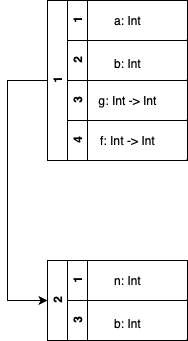
\includegraphics[width=1\linewidth]{Images/ST_example1.png}
  \caption{Symbol table}
\end{subfigure}
\begin{subfigure}{.23\textwidth}
  \centering
  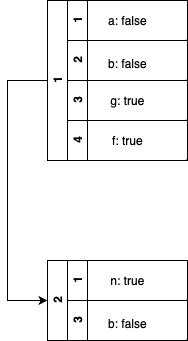
\includegraphics[width=1\linewidth]{Images/VT_example1.png}
  \caption{Var table}
  \label{fig:VTexample}
\end{subfigure}
\caption{ST e VT alla riga 10}
\label{fig:example}
\end{figure}

La ST e VT riga 10 sono mostrate in Figura \ref{fig:example}. Da questa immagine è possibile notare che alle dichiarazioni di funzioni, i loro identificatori vengono salvati nell'ambiente in cui queste vengono dichiarate (in questo caso abbiamo \textit{g} e \textit{f} nell'ambiente 0), quando si entra nel corpo di una funzione viene creato un nuovo ambiente contenente i parametri formali (in questo caso la variabile intera \textit{n}) e gli identificatori degli elementi dichiarati nel corpo della funzione (in questo caso \textit{x}). 

È inoltre utile notare come gli offset siano assegnati agli elementi della ST, il meccanismo è quello di assegnare un valore intero incrementale a partire da 0 in ogni ambiente. Nell'ambiente creato al corpo della funzione verranno prima assegnati i parametri formali, lasciato un offset per il valore di ritorno e solo in seguito vengono assegnati gli elementi dichiarati nel corpo della funzione. 


\subsection{Dichiarazioni multiple}
Per quanto riguarda la gestione degli elementi non dichiarati o dichiarazioni multiple nello stesso ambiente vengono fatti dei controlli durante le dichiarazioni di varibili, funzioni e parametri formali di una stessa funzione.
Nel primo caso si controlla che l'dentificativo utilizzato per la nuova varibile non sia già presente nell'ultimo ambiente della ST (in questo caso viene riportato l'errore), se così non fosse l'identificativo viene aggiunto all'ultimo ambiente della ST. Il controllo è implementato nel nodo \textit{DecvarNode} come segue.
\begin{minted}[xleftmargin=20pt,linenos]{java}
if (ST.top_lookup(id) == true)
        errors.add(new SemanticError("Var id " + id + " already declared"));
    else{
        ST.insert(id, (Type) type, nesting,"") ;
        ST.insertVar(id);
    }
\end{minted}

Nel caso del controllo sulla dichiarazione di funzione e dei suoi paramenti, il controllo eseguito nel nodo \textit{DecfunNode} è il seguente.
\begin{minted}[xleftmargin=20pt,linenos]{java}
if (ST.lookup(id) != null)
    errors.add(new SemanticError("Identifier " + id + " already declared"));
else {
    HashMap<String, STentry> HM = new HashMap<String, STentry>();
    flabel = SimpLanlib.freshFunLabel();
    ST.insert(id, type, nesting, flabel);
    ST.add(HM);
    for (ParNode arg : parlist) {
        if (ST.top_lookup(arg.getId()))
            errors.add(new SemanticError("Parameter id " + arg.getId() +
            " already declared"));
        else {
            ST.insert(arg.getId(), arg.getType(), nesting + 1, "");
        }
    }
    ...
\end{minted}
Come nel caso della dichiarazione di variabile, anche qua si controlla che l'identificativo della funzione non sia presente nell'ultimo ambiente della ST (in questo caso viene riportato l'errore), se così non fosse l'identificativo viene aggiunto all'ultimo ambiente della ST. Solo in seguito viene creato un nuovo ambiente e vengono effettuati i controlli sui paramentri, se questi non sono presenti nell'ultimo (nuovo) ambiente allora vengono aggiunti, altrimenti viene restituito errore. 

\subsection{Identificativi non dichiarati}
Per la gestione degli identificativi non dichiarati sono stati implementati dei controlli sui nodi che richiamano variabili o funzioni, ovvero nel momento in cui viene fatto un assegnamento, espressione che include identificativi o chiamate una fuzione.

Per quanto riguarda il primo caso, il controllo è il seguente e si trova nel nodo \textit{AsgNode}. 
\begin{minted}[xleftmargin=20pt,linenos]{java}
STentry tmp = ST.lookup(id) ;
    if (tmp != null) {
        entry = tmp ; //Se è stato dichiarato allora ok prendo l'entry
    } else { //Se non è stato dichiarato allora errore
        errors.add(new SemanticError("Id " + id + " not declared")) ;
    }
\end{minted}
Prima si recupera l'elemento con identificativo \textit{id} dalla ST, in seguito si controlla se questo elemento sia \textit{null} o meno, nel primo caso si sta provando ad assegnare un'espressione a un elemento non dichiarato, in caso contrario restituisco l'elemento.
Per quanto riguarda le espressioni, bisogna eseguire il controllo nel nodo stesso della variabile, ovvero \textit{IdExpNode}. 
Stessa cosa riguarda la chiamata di funzione, il controllo viene fatto nel nodo \textit{CallNode}. In entrambi i casi, il codice è pressochè simile a quello mostrato precedentemente quindi per semplicità non verrà qui riportato.








%\begin{figure}[h]
%\centering
%\begin{subfigure}{.23\textwidth}
%  \centering
%  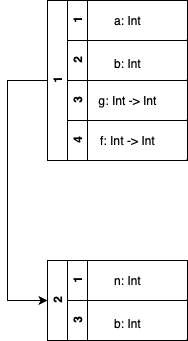
\includegraphics[width=1\linewidth]{Images/ST_example1.png}
%  \caption{Symbol table}
%\end{subfigure}
%\begin{subfigure}{.23\textwidth}
%  \centering
%  \includegraphics[width=1\linewidth]{Images/VT_.png}
%  \caption{Var table}
%\end{subfigure}
%\caption{ST e VT alla riga 9}
%\label{fig:example}
%\end{figure}